\RequirePackage{etex}


\documentclass[11pt]{amsart}

\usepackage{minted}
\usepackage{amsfonts,amssymb,amscd,amsmath,mathrsfs,amsthm}
\usepackage{xcolor}
\usepackage{listings}
\usepackage[utf8]{inputenc}
\usepackage[english]{babel}
\usepackage{amsthm,amsmath,amsfonts,amssymb,amsbsy}
\usepackage{cite,graphicx,color,euscript,epstopdf,url,float}
\usepackage{setspace}
\usepackage{hyperref}
\usepackage{cleveref}
\usepackage{autonum}


% Set the margin and appearance, as set by class standards.
\setlength{\oddsidemargin}{0.25in}  %please do not change
\setlength{\evensidemargin}{0.25in} %please do not change
\setlength{\marginparwidth}{0in} %please do not change
\setlength{\marginparsep}{0in} %please do not change
\setlength{\marginparpush}{0in} %please do not change
\setlength{\topmargin}{0in} %please do not change
\setlength{\footskip}{.3in} %please do not change
\setlength{\textheight}{8.75in} %please do not change
\setlength{\textwidth}{6in} %please do not change
\setlength{\parskip}{4pt} %please do not change

% Add new functions
% Add new function for changing how the equations look
\newcommand{\crefrangeconjunction}{--}

% Change how referencing equations looks
\crefformat{equation}{(#2#1#3)}
\crefrangeformat{equation}{(#3#1#4)--(#5#2#6)}

% Use some standard appearances for math principles
\newtheorem{assumption}{Assumption}[section]
\newtheorem{definition}{Definition}[section]
\newtheorem{theorem}{Theorem}[section]
\newtheorem{lemma}{Lemma}[section]
\newtheorem{proposition}{Proposition}[section]
\newtheorem{corollary}{Corollary}[section]
\newtheorem{remark}{Remark}[section]
\newtheorem{example}{Example}[section]
\newtheorem{algorithm}{Algorithm}[section]
\newtheorem{conjecture}{Conjecture}[section]

\makeatletter
\renewcommand{\@biblabel}[1]{#1.}
\makeatother

\author{Steven~Glasford}
\title{Modeling~warring~fungi~on~a~plant.}
%Title of the first draft
%\title{Numerical Solution of a dynamic equilibrium of pathogen cohorts.}
%The following is the first title that we chose, 
%but we changed it to allow for a shorter and sleeker title.
%%%% Numerical solution of a first-order Hamilton--Jacobi equation for dynamic 
%%%% equilibrium of pathogen cohorts.

\thanks{Advisor: Dr. Ivan Yegorov}
\email{steven.glasford@ndsu.edu}
\address{Department of Mathematics, North Dakota State University, PO Box 6050,
Fargo, ND 58108-6050, USA}

\begin{document}

%The first draft of this paper is due 4 November 2020
\date{Fall~2020}

\maketitle

\begin{abstract}
    In the wild it is very common for fungi and other pathogens to attempt to enter plant hosts, this typically results in competition from other pathogens as well for a single host. Also common is the case when a fungus mutates, where by natural selection, or by the act of introduction into a different environment. This leads to a case where the fungus that has not mutated (the resident) might have to compete with its mutated cousin. In this paper we investigate a zero sum game between a resident and mutant strain of fungi to see if one fungi wins over the other. We also explore the case in which the two strains enter an equilibrium point where both are able to exist. Furthermore, this paper simulates this situation on a single plant for a single season, and does not discuss the potential for evolution between seasons, or the dynamics of multiple plants of the same species.
\end{abstract}


\section{Introduction}
Pathogens are what makes people, pets and every other living organism sick. They are a broad group and can do everything from make a person sick with COVID-19, to blight rotting potatoes in the field starving people. Plant pathogens are everywhere, going outside to the park, it is not uncommon for a person to see brown spots on leaves of trees caused by fungus or to see lichens growing on the bark of oak trees. 

In this paper, a zero-sum feedback game [\ref{terms}.\ref{term:zerosum}] of two competing pathogens on a single plant, battling for dominance on the plant. To do this we use a system of nonlinear ordinary differential equations [\ref{terms}.\ref{term:nonlinearODE}] and use computers and numerical analysis to solve and describe the dynamics of a single growing season of two invading fungal pathogens on a single plant. 

The first fungus can be understood as the resident, while the second is the mutant. The mutant fungus is of the same species, but is a different individual.  The function that describes the invasion of the fungi is the difference between the two marginal fitness criteria [\ref{terms}.\ref{term:marginal}], and represents the cost in defining the  differential game's value [\ref{terms}.\ref{term:differentialgame}].  A general dynamic game approach of \cite{YegorovGrognardMailleretHalkettBernhard2019} is explored and discussed. The Cauchy problem [\ref{terms}.\ref{term:cauchy}] for the first-order Hamilton--Jacobi partial differential equation (HJ PDE) created by this situation is numerically solved using the ROC-HJ software~\cite{ROCHJ2019}. 

Analysis of the numerical simulations obtained by this software package, as well as a graphical description is further investigated later in this document.


\section{Statement of the model}
Before we can properly analyze the numerical solutions we must first define the model. We consider the dynamics of two biotrophic [\ref{terms}.\ref{term:biotrohpic}] fungal cohorts [\ref{terms}.\ref{term:cohort}] on one plant in a single season.  Let us refer to them as to cohorts~$ 1 $ and $ 2 $. For
cohort~$ i $, let $ n_i $ the lesion density, which is the number of mycelia [\ref{terms}.\ref{term:mycelia}]
per unit area of the host. For simplicity, assume $ n_1 $ and $ n_2 $ to be
constant during the entire infection period within the season, which means that
only the resident and the mutant exist on the plant, and there are no new invaders do not penetrate the host during the analyzed period.
In the wild this is  a substantial restriction for infections in, but it still allows for us to draw significant conclusions with relevant
biological interpretations while adhering to standard experimental infection protocols.

We denote the average size of a mycelium in cohort~$ i $ by $ M_i $. and Let $ S_i $
be the average quantity of spores produced by a mycelium in cohort~$ i $. The duration of the
infection ~$ t $ within the season is a time variable. Note that the
mycelial sizes~$ M_1 $ and $ M_2 $ are measured in terms of equivalent amounts
of infecting spores (for instance, if a mycelium appears from one spore at the
beginning of the infection period, the initial mycelial size can be set as one
equivalent of an infecting spore or only as one spore).

To determine the nutrient flux [\ref{terms}.\ref{term:nutrientflux}],
by cohort~$ i $ we use the function,
$ f_i = f_i(M_1, M_2) $, which is allocated between two different pathogen
activities such as within-host multiplication (mycelial growth) and producing
asexual spores. For brevity, we do not explicitly show the dependence on the
constant parameters $ n_1, n_2 $ when writing $ f_i = f_i(M_1, M_2) $,
$ i = 1,2 $. Let $ u_i = u_i(t) $ be a related resource allocation (control)
function, taking values between zero and one. 
When $ u_i(t) = 0 $ the particular fungus only produces mycelia, while when $ u_i(t) = 1 $ the fungus produces spores, and when $ 0 < u_i(t) < 1 $ the fungus is doing both at some degree.
% Suppose that the whole flux goes
% to mycelial growth when $ u_i(t) = 0 $ and to spore production when
% $ u_i(t) = 1 $, while, for $ 0 < u_i(t) < 1 $, there is an intermediate
% configuration. In other words, the fungus expends all of its energy to produce mycelia when 

Let $ g = g(M) $ be the rate of mycelial decay for both cohorts, we assume that the mutation does not. We assume a constant yield of spores, $ \delta > 0 $, as compared to mycelial growth. 

The period of the infections within the season is a fixed interval~$ [0, T] $.

The following dynamic model can thus be formulated 
\cite{YegorovGrognardMailleretHalkettBernhard2019}:
\begin{equation}
\left\{ \begin{aligned}
& \frac{\mathrm{d} M_1(t)}{\mathrm{d} t} \:\: = \:\: \left(1 - u_1(t)\right) \,
  f_1\left(M_1(t), M_2(t)\right) \: - \: g\left(M_1(t)\right), \\
& \frac{\mathrm{d} M_2(t)}{\mathrm{d} t} \:\: = \:\: \left(1 - u_2(t)\right) \,
  f_2\left(M_1(t), M_2(t)\right) \: - \: g\left(M_2(t)\right), \\
& \frac{\mathrm{d} S_1(t)}{\mathrm{d} t} \:\: = \:\: \delta \, u_1(t) \,
  f_1\left(M_1(t), M_2(t)\right), \\
& \frac{\mathrm{d} S_2(t)}{\mathrm{d} t} \:\: = \:\: \delta \, u_2(t) \,
  f_2\left(M_1(t), M_2(t)\right), \\
& M_1(0) = M_1^0, \quad M_2(0) = M_2^0, \quad S_1(0) = S_1^0,
  \quad S_2(0) = S_2^0, \\
& 0 \leqslant u_1(t) \leqslant 1, \quad 0 \leqslant u_2(t) \leqslant 1,
  \quad t \in [0, T].
\end{aligned} \right.  \label{1}
\end{equation}
Since the right-hand sides of the third and fourth equations in (\ref{1}) do
not contain $ S_1 $ and $ S_2 $, one does not need to treat $ S_1 $ and $ S_2 $
explicitly, so that $ M_1 $ and $ M_2 $ can be considered as the only
state variables [\ref{terms}.\ref{term:statevariables}]. %todo: define and cite

The reproductive success (the amount of growth on the plant) of cohort~$ i $ is determined by:
\begin{equation}
\int\limits_0^T \frac{\mathrm{d} S_i(t)}{\mathrm{d} t} \, e^{-\mu t}
    \: dt \:\: = \:\: \delta \,
\int\limits_0^T u_i(t) \, f_i\left(M_1(t), M_2(t)\right) \, e^{-\mu t} \: dt,  \label{3_1}
\end{equation}
where $ e^{-\mu t} $ describes the exponential extinction of the infections as the plant develops immunity,
and $ \mu $ is a positive constant. Since $ \delta $ is a positive constant,
we can divide \cref{3_1} by $ \delta $ and arrive at the following, where $J$ is a Jacobi function [\ref{mathdefs}.\ref{math:jacobi}]

\begin{equation}
J_i\left(u_1(\cdot), u_2(\cdot)\right) \:\: = \:\: \int\limits_0^T u_i(t) \, f_i\left(M_1(t),
  M_2(t)\right) \, e^{-\mu t} \: dt.  \label{3}
\end{equation}


Following with \cite{YegorovGrognardMailleretHalkettBernhard2019,
BernhardGrognardMailleretAkhmetzhanov2010},
we look at the competition between the two cohorts in a single season by investigating their individual reproductive outputs and seeking the saddle control strategies [\ref{terms}.\ref{term:saddlecontrol}] (where the two pathogens enter a sort of ``tie'')
in the following zero-sum two-player differential game:
\begin{equation}
\left\{ \begin{aligned}
& \frac{\mathrm{d} M_1(t)}{\mathrm{d} t} \:\: = \:\: \left(1 - u_1(t)\right) \,
  f_1\left(M_1(t), M_2(t)\right) \: - \: g\left(M_1(t)\right), \\
& \frac{\mathrm{d} M_2(t)}{\mathrm{d} t} \:\: = \:\: \left(1 - u_2(t)\right) \,
  f_2\left(M_1(t), M_2(t)\right) \: - \: g\left(M_2(t)\right), \\
& M_1(0) = M_1^0, \quad M_2(0) = M_2^0, \\
& 0 \leqslant u_1(t) \leqslant 1, \quad 0 \leqslant u_2(t) \leqslant 1,
  \quad t \in [0, T],
\end{aligned} \right.  \label{7}
\end{equation}
\begin{equation}
J(u_1(\cdot), u_2(\cdot)) \:\: \longrightarrow \:\: 
\inf_{u_1(\cdot)} \:  \sup_{u_2(\cdot)} 
\:\: \mbox{or} \:\:
\sup_{u_2(\cdot)} \: \inf_{u_1(\cdot)} \, ,  \label{8}
\end{equation}
\begin{equation}
\begin{aligned}
& J\left(u_1(\cdot), u_2(\cdot)\right) \:\: = \:\: J_2\left(u_1(\cdot), u_2(\cdot)\right) \: - \:
J_1\left(u_1(\cdot), u_2(\cdot)\right) \\
& \quad
= \:\: \int\limits_0^T \left( u_2(t) \, f_2(M_1(t), M_2(t)) \: - \: u_1(t)
  \, f_1(M_1(t), M_2(t)) \right) \,
e^{-\mu t} \: dt.
\end{aligned}  \label{9}
\end{equation}
Where $\inf$ is the infimum [\ref{mathdefs}.\ref{math:infimum}] and $\sup$ is the supremum [\ref{mathdefs}.\ref{math:supremum}].


According to \cite{YegorovGrognardMailleretHalkettBernhard2019}, we represent
the nutrient fluxes [\ref{terms}.\ref{term:nutrientflux}] and decay rates as

\begin{equation}
f_i(M_1, M_2) \: = \: \nu(n_1 M_1 + n_2 M_2) \, \cdot \, \rho(M_i) \:\:\:
\forall M_1 \geqslant 0 \:\:\: \forall M_2 \geqslant 0, \quad i = 1,2, 
  \label{4}
\end{equation}
\begin{equation}
\rho(M) \: = \: \alpha \: \dfrac{M}{M + k} \quad \forall M \geqslant 0, 
  \label{5_1}
\end{equation}
\begin{equation}
\nu(n_1 M_1 + n_2 M_2) \: = \: \dfrac{1}{1 + \beta \, (n_1 M_1 + n_2 M_2)}
  \quad
\forall M_1 \geqslant 0 \quad \forall M_2 \geqslant 0,  \label{5_2}
\end{equation}
\begin{equation}
g(M) \: = \: \gamma M \quad \forall M \geqslant 0.  \label{6}
\end{equation}
Where $\rho$ is a positive function that specifies the flow of resources obtained by a single mycelium, and $\nu$ describes the negative consequences as the pathogens compete for resources from the single plant  \cite{YegorovGrognardMailleretHalkettBernhard2019}.

Furthermore, the following parameter values are also useful for the numerical
simulations and arise from the analysis of
\cite{YegorovGrognardMailleretHalkett2017}:
\begin{equation}
\arraycolsep=1.3pt
\def\arraystretch{1.5}
\begin{array}{c}
\alpha \: = \: 0.2 \cdot 10^4 \:\: \mathrm{spores} / \mathrm{day}, \quad
k \: = \: (1/6) \cdot 10^4 \:\: \mathrm{spores}, \\
\beta \: = \: 10^{-5} \:\: \mathrm{cm}^2 / \mathrm{spores}^2, \quad \gamma
  \: = \: 0.06 \:\: 1 / \mathrm{day}, \quad
\mu \: = \: 0.03 \:\: 1 / \mathrm{day}, \\
n_1 \: = \: 9 \:\: \mathrm{spores} / \mathrm{cm}^2, \quad n_2 \: = \: 1 \:\:
  \mathrm{spore} / \mathrm{cm}^2, \\
T \: = \: 60 \:\: \mathrm{days}.
\end{array}  \label{19}
\end{equation}

As was shown in \cite{YegorovGrognardMailleretHalkettBernhard2019}, the bounded
domain
\begin{equation}
G \:\: = \:\: \left\{ (M_1, M_2) \: \in \: \mathbb{R}^2 \: \colon \: 0 < M_1 <
  \bar{M}_1, \:
0 < M_2 < \bar{M}_2 \right\}  \label{2}
\end{equation}
with
\begin{equation}
\bar{M}_1 \: = \: \bar{M}_2 \: > \: \alpha / \gamma - k  \label{2_1}
\end{equation}
is an invariant set in the state space (if a state trajectory starts in $ G $,
it cannot leave $ G $). The parameters~$ \bar{M}_1, \bar{M}_2 $ can be
understood as 
carrying capacity [\ref{terms}.\ref{term:carryingcapacity}] estimates. 


\section{Uninvadable and evolutionarily stable strategies}
In war there are times in which neither party wins. Where there is a boundary or other concession exist, under this circumstance the resident is uninvadable. In this section we describe the strategies and functions used to model a stable and uninvadable resident pathogen, in other words we see see were the two pathogens enter a stalemate and we look deeper at the game-theoretic statements from {\rm \cref{7,8,9}}.

Based on the terminology of Adaptive Dynamics \cite{DercoleRinaldi2008}, let
us interpret cohort~{\rm 1} as a resident and cohort~{\rm 2} as a mutant.
Denote the corresponding classes of considered strategies as $ \mathcal{U}_1 $
and $ \mathcal{U}_2 $. For a pair of methods
$ \: (u_1, u_2) \, \in \, \mathcal{U}_1 \times \mathcal{U}_2, \: $
the resident is not invaded by the mutant if and only if
$$
J(u_1, u_2) \: = \: J_2(u_1, u_2) - J_1(u_1, u_2) \: \leqslant \: 0.
$$
A strategy 
$ \hat{u}_1 \in \mathcal{U}_1 $
is hence uninvadable, and the winner of the war is the resident if and only if
$$
J \left( \hat{u}_1, u_2 \right) \: \leqslant \: 0 \quad \forall u_2 \in
  \mathcal{U}_2,
$$
which is equivalent to
$$
\sup_{u_2 \, \in \, \mathcal{U}_2} \: J \left( \hat{u}_1, u_2 \right) \:\:
  \leqslant \:\: 0
$$
where $\sup$ is the supremum [\ref{mathdefs}.\ref{math:supremum}].


Such a $ \hat{u}_1 $ exists if
\begin{equation}
\inf_{u_1 \, \in \, \mathcal{U}_1} \: \sup_{u_2 \, \in \, \mathcal{U}_2} \:
  J(u_1, u_2) \:\: = \:\:
\min_{u_1 \, \in \, \mathcal{U}_1} \: \sup_{u_2 \, \in \, \mathcal{U}_2} \:
  J(u_1, u_2) \:\: \leqslant \:\: 0  \label{9_2}
\end{equation}
or
\begin{equation}
\inf_{u_1 \, \in \, \mathcal{U}_1} \: \sup_{u_2 \, \in \, \mathcal{U}_2} \:
  J(u_1, u_2) \:\: < \:\: 0  \label{9_4}
\end{equation}
(The latter inequality arises from when the infimum [\ref{mathdefs}.\ref{math:infimum}] $u_1$ is not satisfied).
Equation \cref{9_2} motivates our game-theoretic statement~{\rm \cref{7,8,9},}
where the first player tries to maximize its resistance to an invasion by the
second one{\rm ,} and vice versa. In other words, the resident fungus tries to grow and fight the opposing mutant fungus, and the mutant fungus tries to do the same.

If $ M_1^0 = M_2^0 $ and $ \mathcal{U}_1 = \mathcal{U}_2 = \mathcal{U} ${\rm ,}
then $ J(u, u) = 0 $ for all $ u \in \mathcal{U} ${\rm ,} and {\rm (\ref{9_2})}
is simplified to

%todo: define Arg or remove if meaningless
\begin{equation}
\min_{u_1 \, \in \, \mathcal{U}} \: \sup_{u_2 \, \in \, \mathcal{U}} \:
  J(u_1, u_2) \:\: = \:\: 0  \label{9_3}
\end{equation}


This is the boundary where neither the resident and the mutant win, and there is a stalemate.
In this case{\rm ,} a strategy

$$
\hat{u}_1 \:\: \in \:\: \mathrm{Arg} \min_{u_1 \, \in \, \mathcal{U}}
  \left( \sup_{u_2 \, \in \, \mathcal{U}} \: J(u_1, u_2) \right)
$$

where $\mathrm{Arg} \min$ is the argument of the minimum [\ref{mathdefs}.\ref{math:Argmaxmin}]. The strategy is called evolutionary stable, and there is a boundary where neither pathogen wins if the related maximum for $ u_2 $ is
unique:
$$
\mathrm{Arg} \max_{u_2 \, \in \, \mathcal{U}} \: J \left( \hat{u}_1, u_2
  \right) \:\: = \:\: \left\{ \hat{u}_1 \right\}.
$$
where $\mathrm{Arg}\max$ is the argument of the maximum [\ref{mathdefs}.\ref{math:Argmaxmin}]


This approach to defining stable evolutionary strategies was initially proposed
in \cite{BernhardGrognardMailleretAkhmetzhanov2010} and further developed
in \cite{YegorovGrognardMailleretHalkettBernhard2019}.


\section{Hamilton--Jacobi--Isaacs equation}
In order to determine how the evolutionary strategies change over time we must develop a system of differential functions. This circumstance is very well able to be solved using a Hamilton--Jacobi-Isaacs equation, and for brevity we exclude the reasoning behind using this, but more information and futher analysis can be found in \cite{YegorovGrognardMailleretHalkettBernhard2019}.

We introduce the following function known as Hamiltonian:
\begin{equation}
\begin{aligned}
& H(t, M_1, M_2, u_1, u_2, p_1, p_2) \:\: = \:\:
p_1 \, \left((1 - u_1) \, f_1(M_1, M_2) \: - \: g(M_1)\right) \\
& \qquad\qquad\qquad\qquad\qquad\quad \:\:\:\,
+ \:\: p_2 \, \left((1 - u_2) \, f_2(M_1, M_2) \: - \: g(M_2)\right) \\
& \qquad\qquad\qquad\qquad\qquad\quad \:\:\:\,
+ \:\: e^{-\mu t} \, (u_2 \, f_2(M_1, M_2) \: - \: u_1 \, f_1(M_1, M_2)) \\
& \forall t \in [0, T] \quad \forall \: (M_1, M_2) \: \in \: G \quad \forall
  \: (u_1, u_2) \: \in \: [0, 1]^2 \quad
\forall \: (p_1, p_2) \: \in \: \mathbb{R}^2
\end{aligned}  \label{12}
\end{equation}
(this is the sum of the dot product of $ \: p = (p_1, p_2) \: $ with
$ \: (\mathrm{d} M_1 / \mathrm{d} t, \, \mathrm{d} M_1 / \mathrm{d} t) \: $ and
the integrand in $ \: J(u_1(\cdot), u_2(\cdot)), \: $ see \cref{7} and
%%%%%%%%%%%%%%%%%%%%%%%%%%%
\cref{9}). The Hamiltonian satisfies the saddle point condition [\ref{mathdefs}.\ref{math:saddlepoint}] concerning
the control variables~$ u_1 $ and
$ u_2 $
\begin{equation}
\begin{aligned}
& \min_{u_1 \in [0, 1]} \: \max_{u_2 \in [0, 1]} \: H(t, M_1, M_2, u_1, u_2,
  p_1, p_2) \\
& \qquad
= \:\: \max_{u_2 \in [0, 1]} \: \min_{u_1 \in [0, 1]} \: H(t, M_1, M_2, u_1,
  u_2, p_1, p_2) \:\:
= \:\: \mathcal{H} (t, M_1, M_2, p_1, p_2) \\
& \forall t \in [0, T] \quad \forall \: (M_1, M_2) \: \in \: G \quad \forall
  \: (p_1, p_2) \: \in \: \mathbb{R}^2
\end{aligned}  \label{13}
\end{equation}
(here minimax and maximin [\ref{mathdefs}.\ref{math:maximinminimax}] give the same result). Due to the theoretical
results of \cite[\S XI.6]{FlemingSoner2006}, the value function [\ref{mathdefs}.\ref{math:valuefunction}]
$ \: V \colon [0, T] \times G \to \mathbb{R} \: $ in the formulated feedback

differential game is a unique solution of the following Cauchy problem [\ref{mathdefs}.\ref{math:cauchyproblem}] for the
Hamilton--Jacobi--Isaacs partial differential equation (HJI PDE):
\begin{equation}
\left\{ \begin{aligned}
& \frac{\partial V(t, M_1, M_2)}{\partial t} \: + \: \mathcal{H}
  \left( t, M_1, M_2, \frac{\partial V(t, M_1, M_2)}{\partial M_1},
  \frac{\partial V(t, M_1, M_2)}{\partial M_2} \right) \:\: = \:\: 0, \\
& V(T, M_1, M_2) \: = \: 0, \\
& t \in [0, T], \quad (M_1, M_2) \: \in \: G.
\end{aligned} \right.  \label{15}
\end{equation}

In general, the solution may be 
nonsmooth [\ref{mathdefs}.\ref{math:nonsmooth}] and understood in a generalized (viscosity [\ref{mathdefs}.\ref{math:viscosity}] or minimax) sense \cite{FlemingSoner2006,Subbotin1995}. This makes it difficult, if not impossible to solve precisely.

Due to the general properties of value functions of zero-sum feedback
differential games \cite{BotkinHoffmannTurova2011}, the value function~$ V $
in our problem is limited in how fast it can change and is therefore Lipschitz continuous [\ref{mathdefs}.\ref{math:lipschitz}] in $ [0, T] \times G $. 
Rademacher's theorem [\ref{mathdefs}.\ref{math:rademacher}],
is differentiable almost everywhere in $ (0, T) \times G $, except
for possibly a 
subset of Lebesgue measure zero. 

For points~$ (t, M_1, M_2) $ at which the value function is differentiable,
one can obtain the saddle feedback control strategies (where the fungi enter a stalemate) from the relations
$$
\begin{aligned}
& u_1(t, M_1, M_2) \:\: \in \:\: \mathrm{Arg} \min_{w_1 \in [0, 1]}
  \left\{ \max_{w_2 \in [0, 1]} \:
H \left( t, M_1, M_2, w_1, w_2, {}^{{}^{{}^{{}^{{}^{}}}}} \right. \right. \\
& \qquad\qquad\qquad\qquad\qquad\qquad\qquad\qquad\qquad
\left. \left. \frac{\partial V(t, M_1, M_2)}{\partial M_1}, \,
  \frac{\partial V(t, M_1, M_2)}{\partial M_2} \right) \right\}, \\
& u_2(t, M_1, M_2) \:\: \in \:\: \mathrm{Arg} \max_{w_2 \in [0, 1]}
  \left\{ \min_{w_1 \in [0, 1]} \:
H \left( t, M_1, M_2, w_1, w_2, {}^{{}^{{}^{{}^{{}^{}}}}} \right. \right. \\
& \qquad\qquad\qquad\qquad\qquad\qquad\qquad\qquad\qquad
\left. \left. \frac{\partial V(t, M_1, M_2)}{\partial M_1}, \,
  \frac{\partial V(t, M_1, M_2)}{\partial M_2} \right) \right\},
\end{aligned}
$$
which reduce to
\begin{equation}
\begin{aligned}
& u_1(t, M_1, M_2) \:\: = \:\: \begin{cases}
0, & e^{-\mu t} \: + \: \frac{\partial V(t, M_1, M_2)}{\partial M_1}
  \: < \: 0, \\
1, & e^{-\mu t} \: + \: \frac{\partial V(t, M_1, M_2)}{\partial M_1}
  \: > \: 0, \\
\mbox{arbitrary from} \:\: [0, 1], & e^{-\mu t} \: + \: \frac{\partial
  V(t, M_1, M_2)}{\partial M_1} \: = \: 0,
\end{cases} \\
& u_2(t, M_1, M_2) \:\: = \:\: \begin{cases}
0, & e^{-\mu t} \: - \: \frac{\partial V(t, M_1, M_2)}{\partial M_2}
  \: < \: 0, \\
1, & e^{-\mu t} \: - \: \frac{\partial V(t, M_1, M_2)}{\partial M_2}
  \: > \: 0, \\
\mbox{arbitrary from} \:\: [0, 1], & e^{-\mu t} \: - \: \frac{\partial V(t,
M_1, M_2)}{\partial M_2} \: = \: 0.
\end{cases}
\end{aligned}  \label{16}
\end{equation}
These are resource allocation strategies and functions that describe the equilibrium point and the coexistence of the two fungi. In other words, these equations describe the points where the two fungi enter a stalemate dynamically as time progresses. 

%%%%%%%%%%%%%%%%%%%%%1 
%todo: merge code section with the numerical solution section, or add the code section after the numerical solution section
\section{Code used for the Numerical Solution.}

As described previously, these equations are extremely difficult to solve precisely, luckily, we do not necessarily need a precise answer. Numerical analysis is the math behind finding such answers of difficult to solve problems. In our case there is already a program to solve Hamilton--Jacobi equations called ROC-HJ, which is written in C++ and allows for a fast and easy
transcription of the functions above into machine code. 

Most of the preconfigured files and procedures of ROC-HJ allow for a quick transcription
of a Hamilton-Jacobi equation. More information about how to install ROC-HJ and were to find the package can be found at \cite{ROCHJ2019} and it also has large amount of documentation providing further details of the type of assignments and
other variables that need additional configuration in order for ROC-HJ to find
a solution. To use ROC-HJ, we must assign a few variables to describe the kind
of problem. Fig. \ref{code:defaults} contains some of the variables which
describe the problem.


With these as well as many more options that we had to set to correctly assign
the type of problem that we needed for the system to function precisely, we
also needed to specify both a cost function (fig. \ref{code:cost}) and a
dynamic equation (fig. \ref{code:dynamic}) to produce the data that we need.


Within the \texttt{data\_*.h} file, there is much more information describing
the function. One can find more information and details about this project's
configuration variables by viewing the data file directly at \cite{data_ivan.h}.

\section{Numerical solution}
%todo: add motivation

We consider the Cauchy problem~\cref{15} for the HJI PDE with the nutrient
fluxes~\cref{4,5_1,5_2}, decay rate~\cref{6}, and parameter values~\cref{19}.
The numerical solution has been obtained via a finite difference method
\cite{FlemingSoner2006,
      OsherShu1991,
      BotkinHoffmannTurova2011,
      BokanForcadelZidani2010}
using the ROC-HJ software~\cite{ROCHJ2019}.

For practical purposes, it is reasonable to rewrite \cref{15} in reverse
time $ \tau = T - t $ as
\begin{equation}
\left\{ \begin{aligned}
& \frac{\partial V(T - \tau, M_1, M_2)}{\partial \tau} \:\: + \:\:
\max_{u_1 \in [0, 1]} \: \min_{u_2 \in [0, 1]} \:
\left( -H \left( T - \tau, \, M_1, \, M_2, \, u_1, \, u_2, 
{}^{{}^{{}^{{}^{{}^{}}}}} \right. \right. \\
& \qquad\qquad\qquad\qquad\qquad
\left. \left. \frac{\partial V(T - \tau, M_1, M_2)}{\partial M_1}, \,
\frac{\partial V(T - \tau, M_1, M_2)}{\partial M_2} \right) \right) \:\: =
\:\: 0, \\
& V(T - \tau, M_1, M_2) \left|_{\tau = 0} \right. \: = \: 0, \\
& \tau \in [0, T], \quad (M_1, M_2) \: \in \: G,
\end{aligned} \right.  \label{75}
\end{equation}
and then to rewrite (\ref{75}) in the new normalized state variables
\begin{equation}
m_i \, = \, M_i \cdot 10^{-4}, \quad i = 1,2  \label{75_1}
\end{equation}
(such changes of the time and state variables lead to an equivalent problem).

We specify the carrying capacity estimates as $ \: \bar{M}_1 = \bar{M}_2 =
\bar{M} = 3.5 \cdot 10^4 $,
$ \: \bar{m} = \bar{M} \cdot 10^{-4} = 3.5, \: $ and 
discretize the computational region %todo: add more details and explain
$$
\left\{ (m_1, m_2, \tau) \: \colon \: 0 \leqslant m_1 \leqslant \bar{m}, \:\: 0
\leqslant m_2 \leqslant \bar{m}, \:\:
0 \leqslant \tau \leqslant T \right\}
$$
by the spatial step $ \: \Delta m_1 = \Delta m_2 = \Delta m = 2 \cdot 10^{-3}
\: $ and time step $ \Delta \tau = 5 \cdot 10^{-3} $.

Monotone finite difference methods %todo: cite and explain
(including the 
classical Lax--Friedrichs scheme %todo: define and cite
) ensure theoretical convergence properties with error estimates, but
they are mostly of the first order and may generate so-called 
numerical diffusion problems %todo: define and cite
on long time intervals. One way to attenuate such practical
issues is to use 
higher-order ENO (essentially non-oscillatory) schemes %todo: define and cite
such as those originally proposed in \cite{OsherShu1991}. They are not necessarily
monotone, and there is a lack of associated convergence theorems. However,
their relevance is justifiable by various numerical experiments 
\cite{OsherShu1991,BokanForcadelZidani2010}.

We have used the second-order ENO scheme (to approximate the partial
derivatives concerning the state variables), coupled with the 
second-order Runge--Kutta time discretization scheme %todo: cite and explain
and implemented in \cite{ROCHJ2019}.
To evaluate the partial derivatives $ \partial V / \partial M_i $, $ i = 1,2 $,
in the saddle feedback control representations~\cref{16}, we have applied the
standard second-order symmetrized approximation
\cite[\S 5.7]{PressTeukolskyVetterlingFlannery2007}.

Figs.~\ref{Fig_4} and \ref{Fig_5} show the reductions of the approximate
value function and corresponding saddle feedback control strategies to the
coordinate plane $ (m_1, m_2) $ for the time instants 
$ \tau = 0 $ ($ t = T = 60 $), $ \tau = 5 $ ($ t = T - 5 = 55 $),
$ \tau = \tau^{**} %todo: define or explain tau**
\approx 11.175 $ ($ t = T - \tau^{**} \approx 48.825 $),
and $ \tau = T = 60 $ ($ t = 0 $). Here $ \tau^{**} $ is a 
reverse time instant %todo: define and cite
that triggers the appearance of singular control regimes and is obtained
together with the equilibrium steady state~$ \left( M^{**}, M^{**} \right) $
from the analysis based on 
Pontryagin's principle %todo: explain and maybe cite (cones and hyperplanes)
\cite{YegorovGrognardMailleretHalkettBernhard2019}. Note that Pontryagin's
principle for zero-sum two-player differential games describes necessary
conditions for saddle open-loop strategies \cite{Yong2015}.

\begin{figure}
\center{ 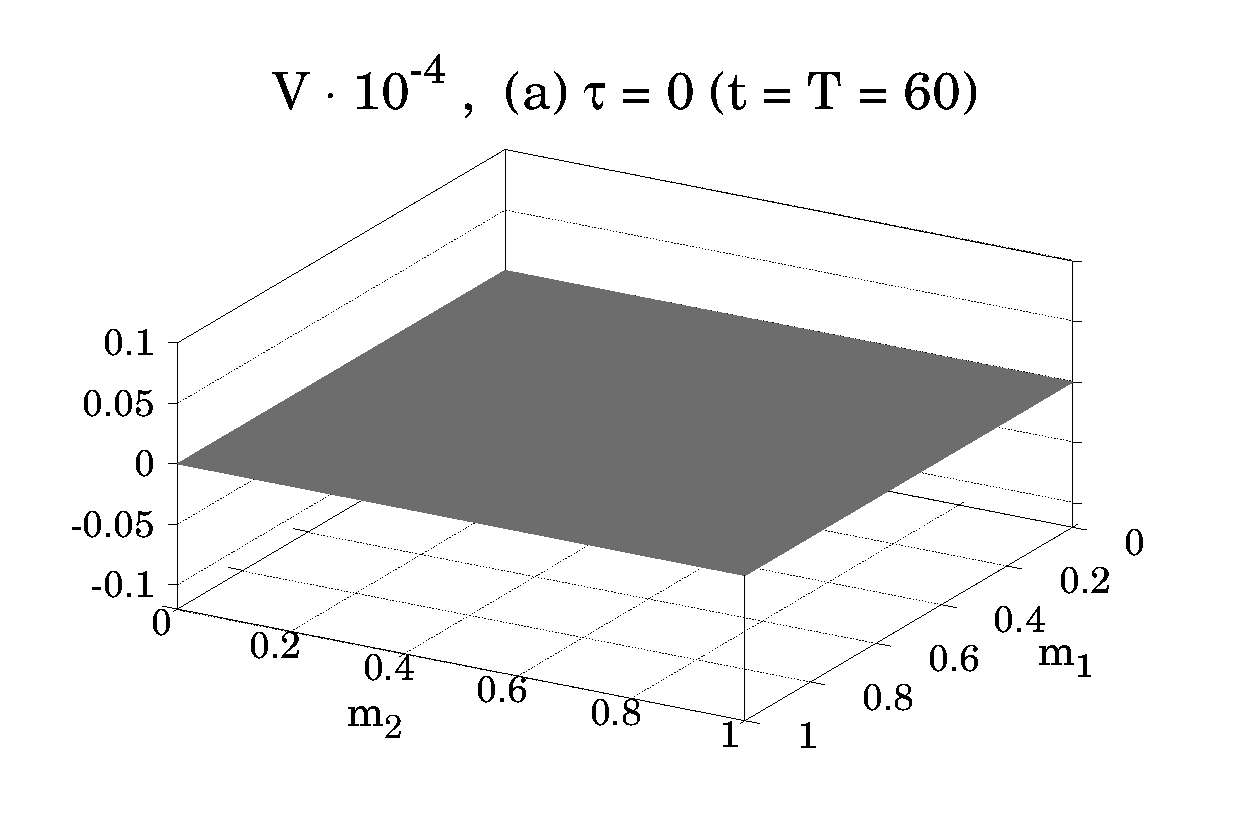
\includegraphics[width = 0.48 \textwidth]{figures/Figure_4a.pdf}
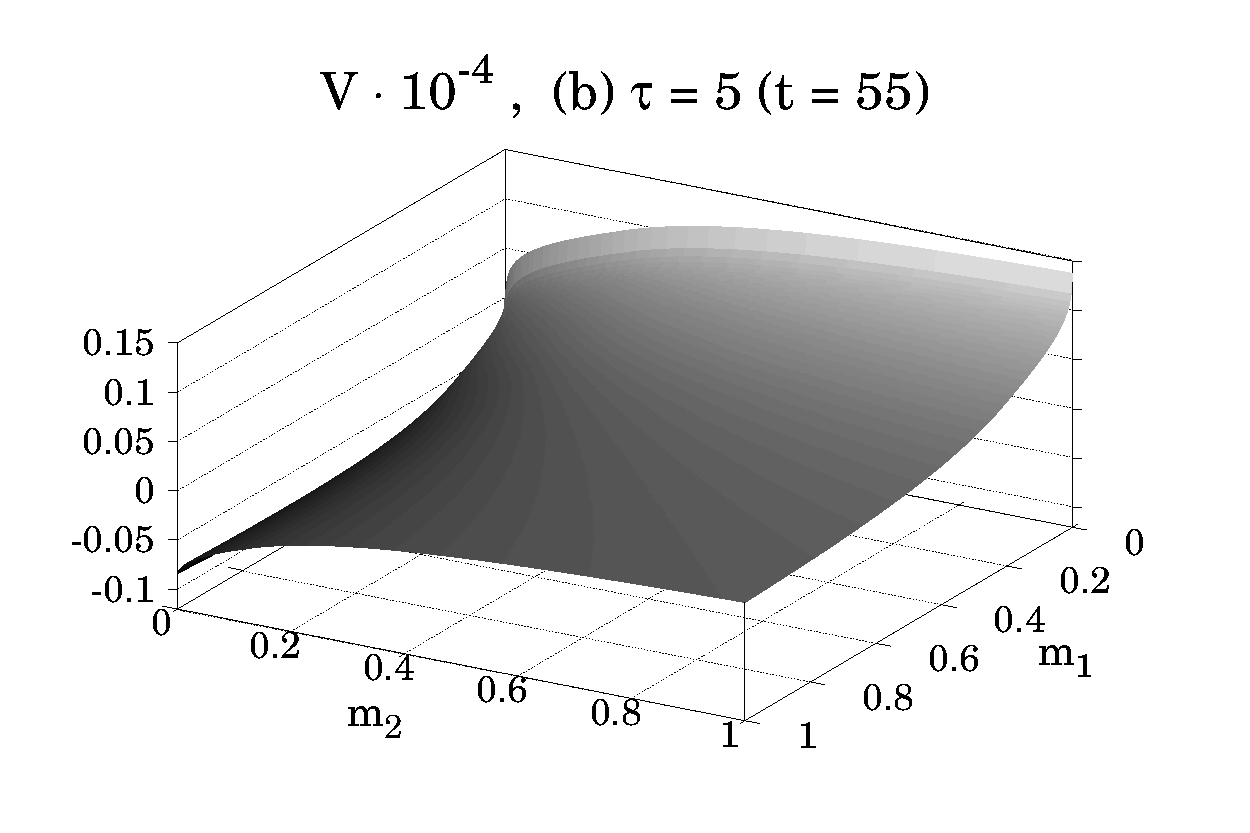
\includegraphics[width = 0.48 \textwidth]{figures/Figure_4b_1.pdf} \\
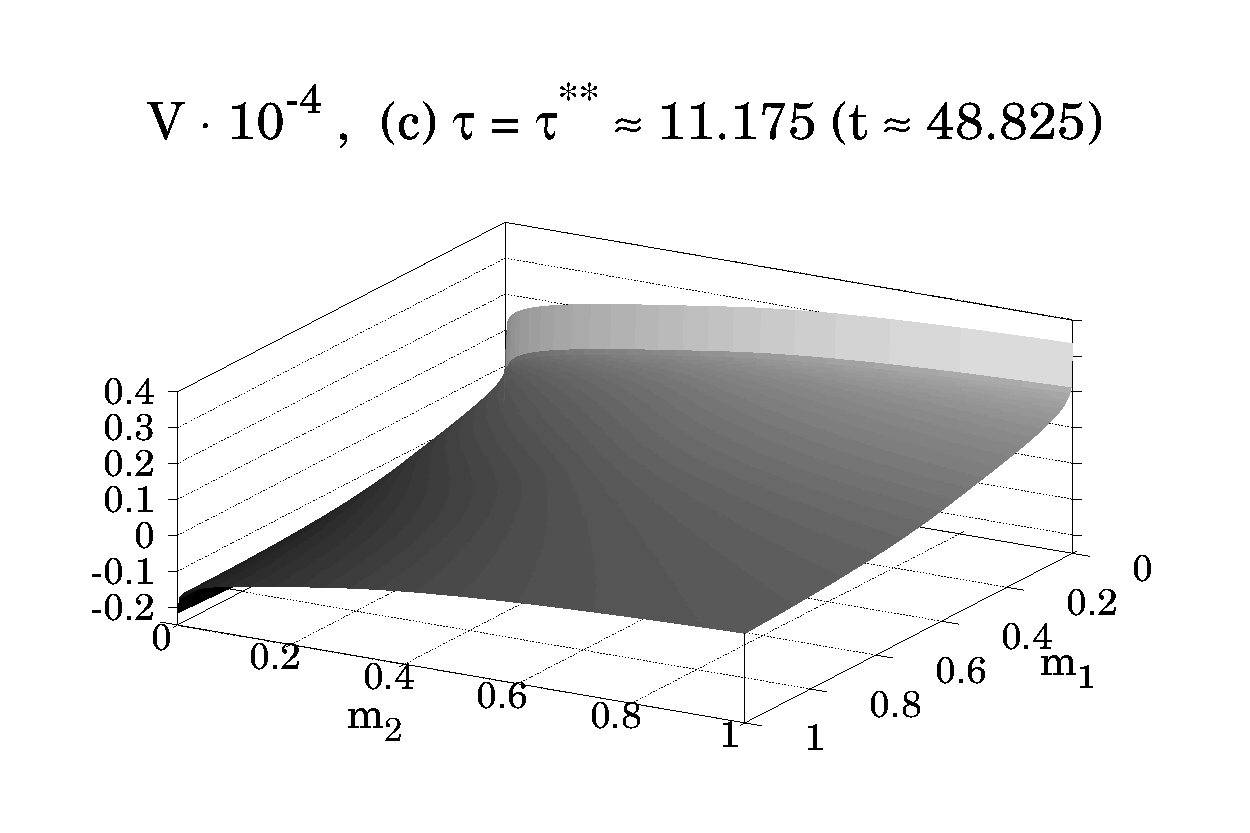
\includegraphics[width = 0.48 \textwidth]{figures/Figure_4c_1.pdf}
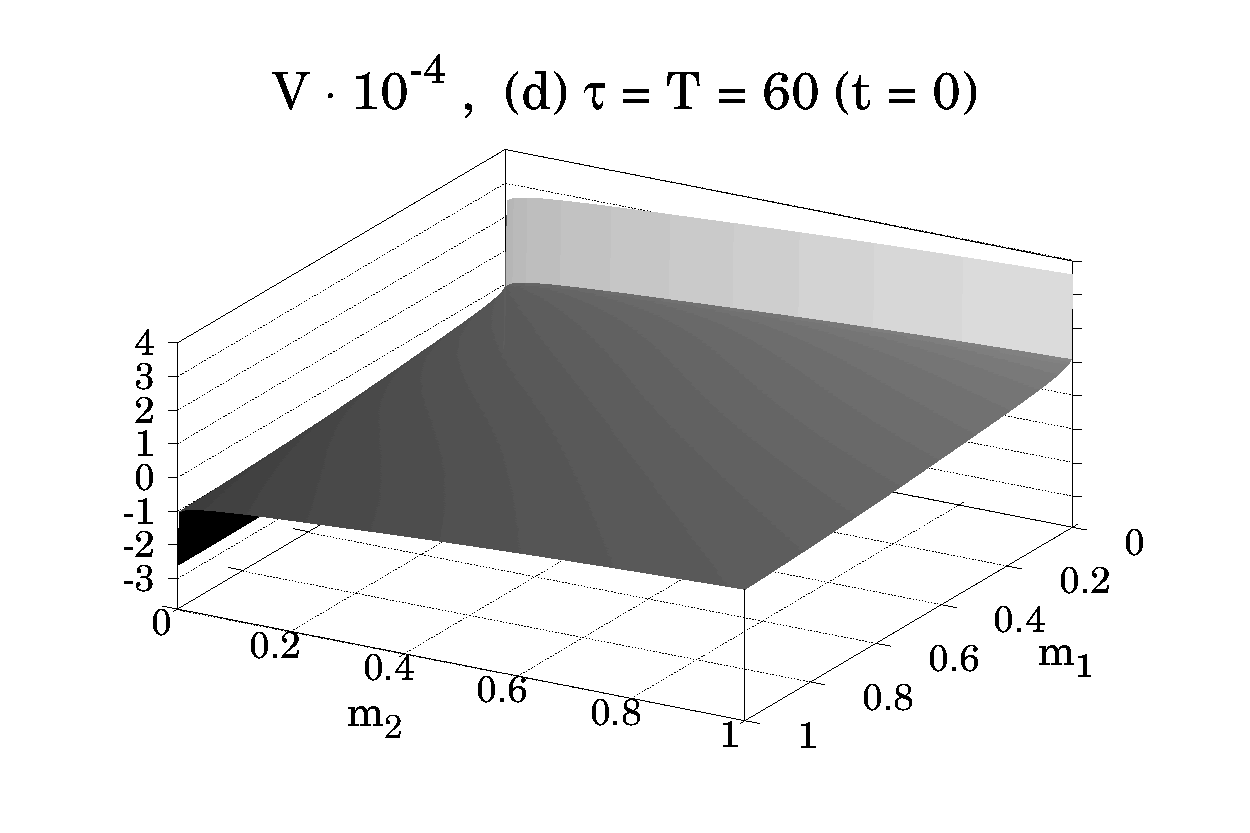
\includegraphics[width = 0.48 \textwidth]{figures/Figure_4d_1.pdf}
}
\bf \caption{\it Finite-difference approximation of the value function~$ V $
                 at several time instants.}
\label{Fig_4}
\end{figure}

\begin{figure}
\center{ 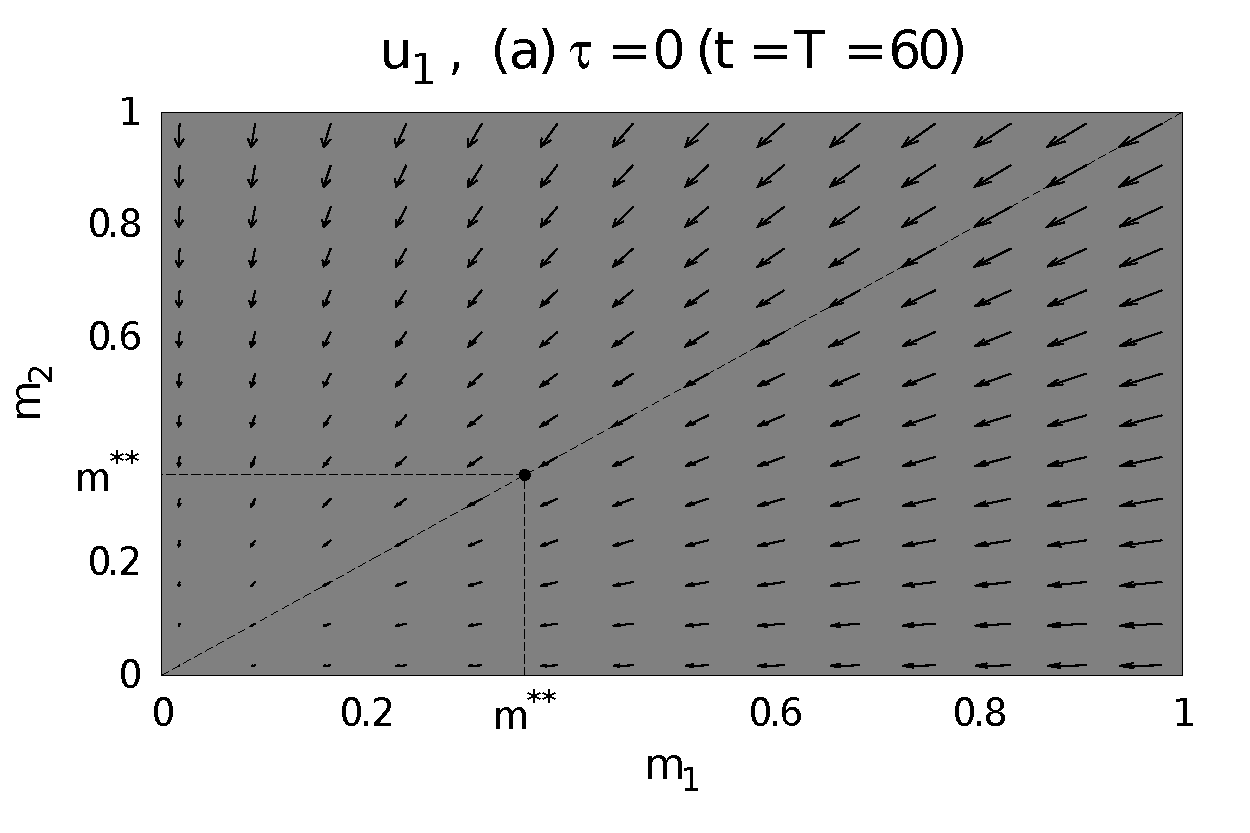
\includegraphics[width = 0.48 \textwidth]{figures/Figure_5a_1.pdf}
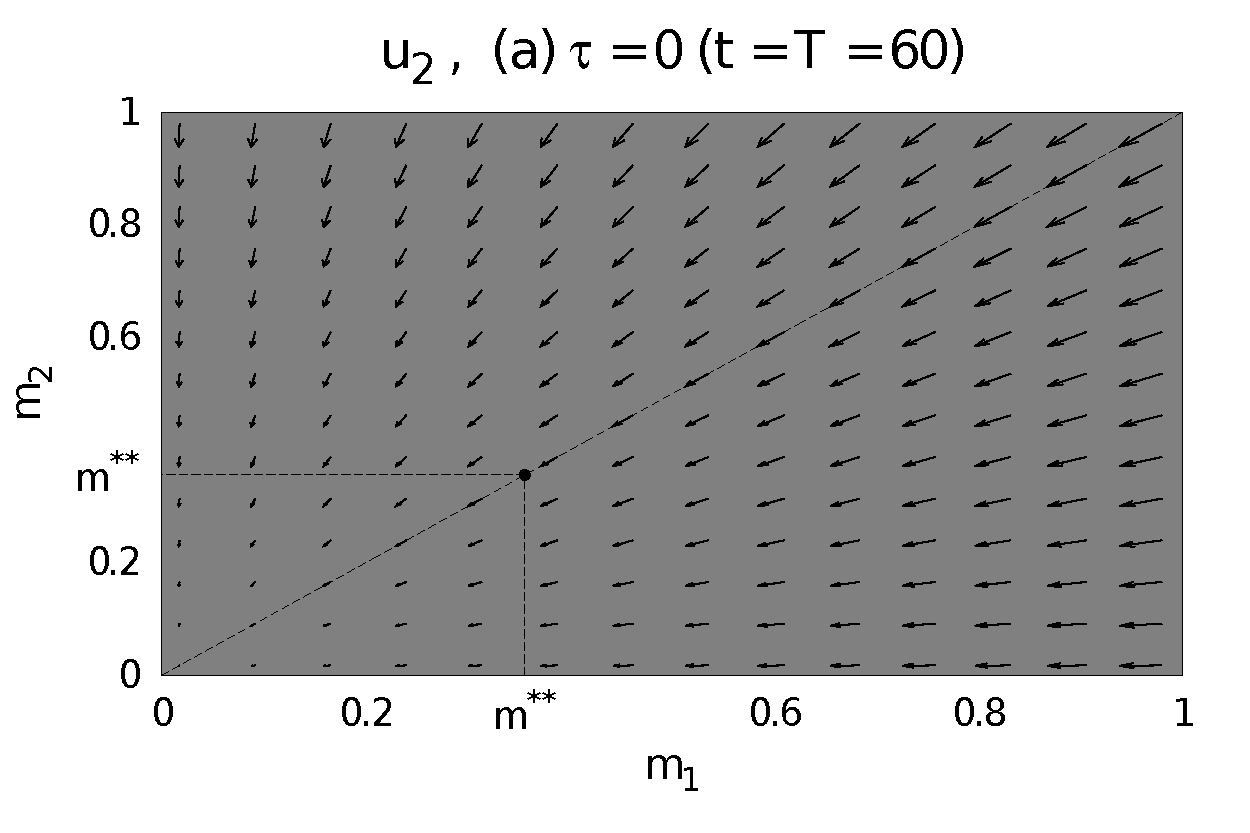
\includegraphics[width = 0.48 \textwidth]{figures/Figure_5a_2.pdf} \\
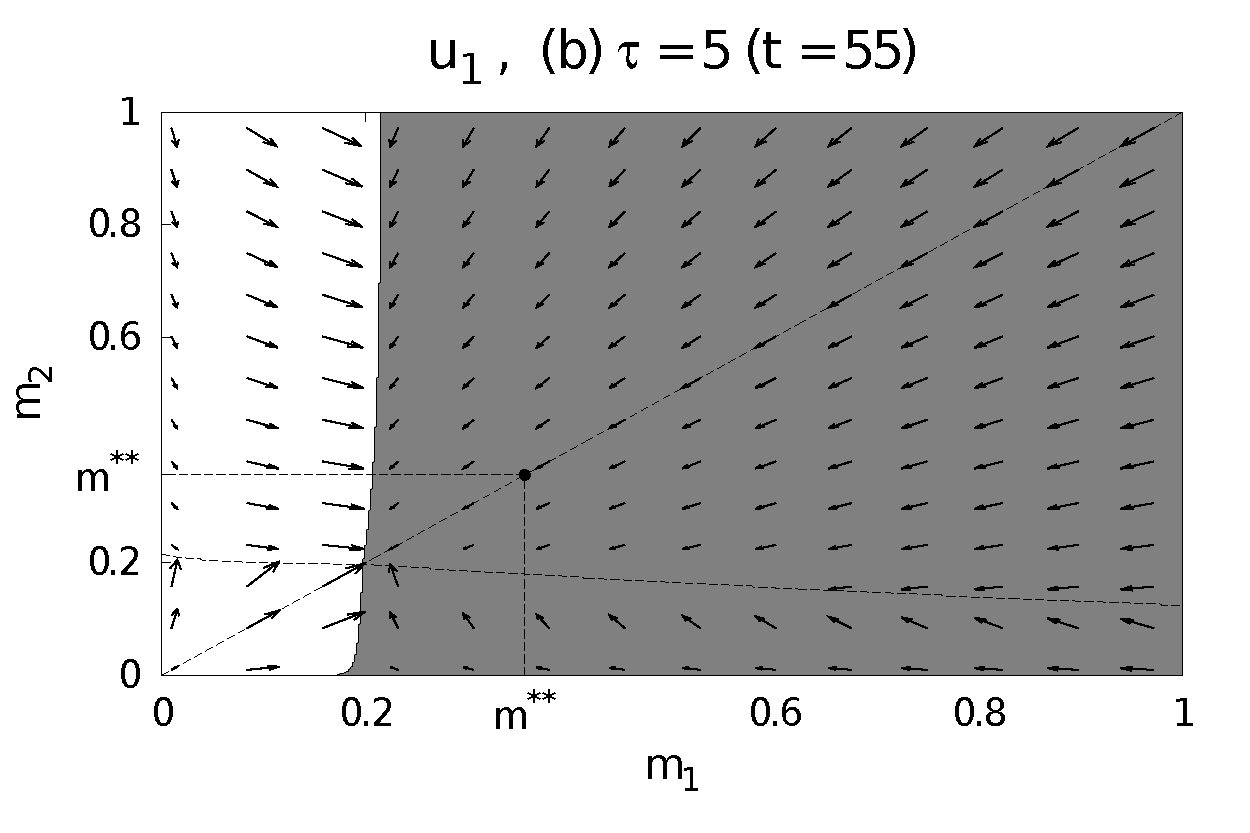
\includegraphics[width = 0.48 \textwidth]{figures/Figure_5b_1.pdf}
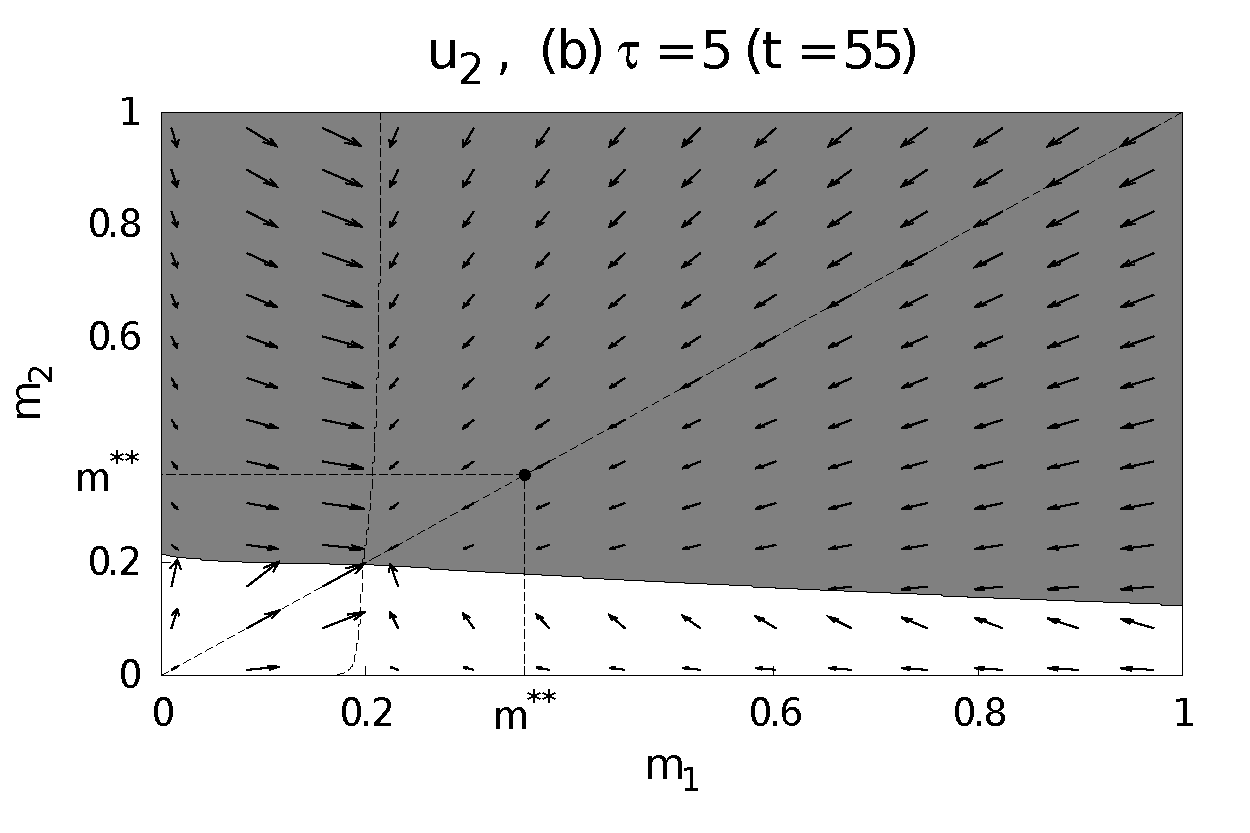
\includegraphics[width = 0.48 \textwidth]{figures/Figure_5b_2.pdf} \\
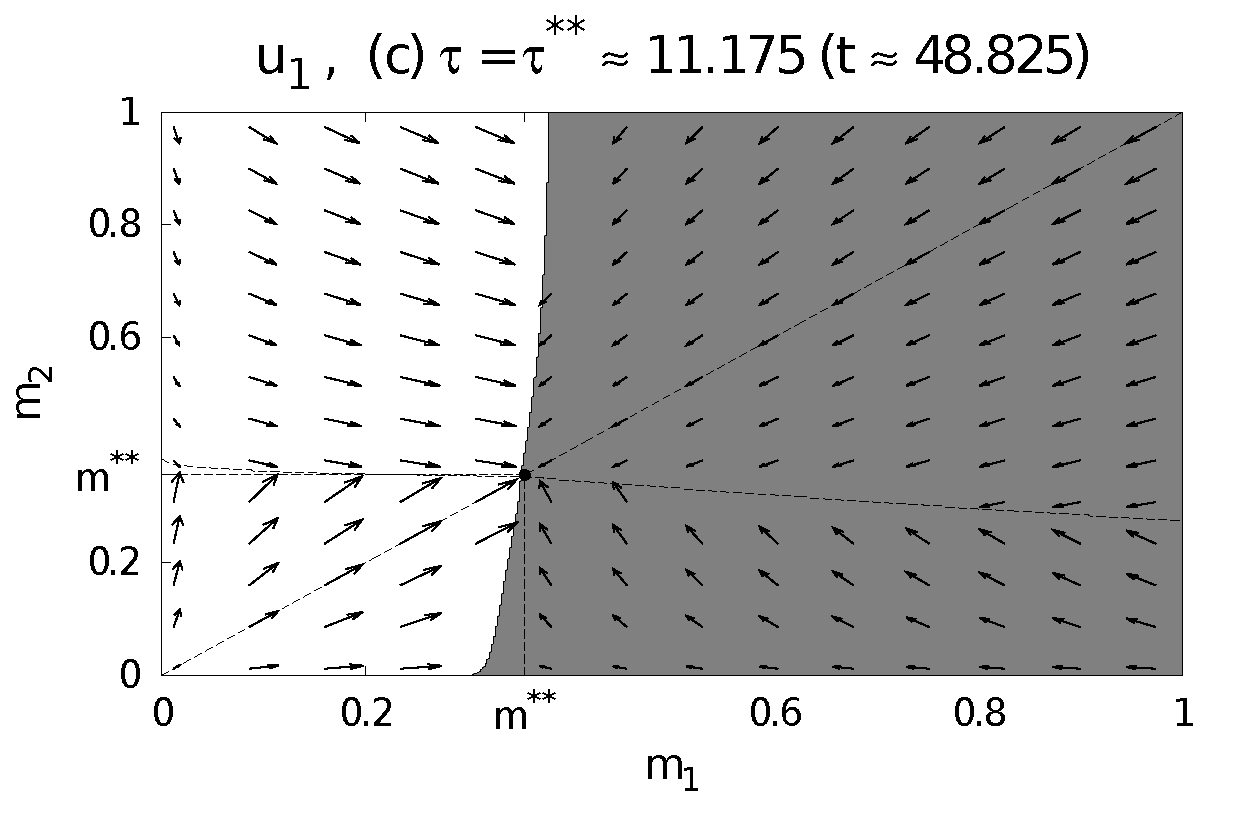
\includegraphics[width = 0.48 \textwidth]{figures/Figure_5c_1.pdf}
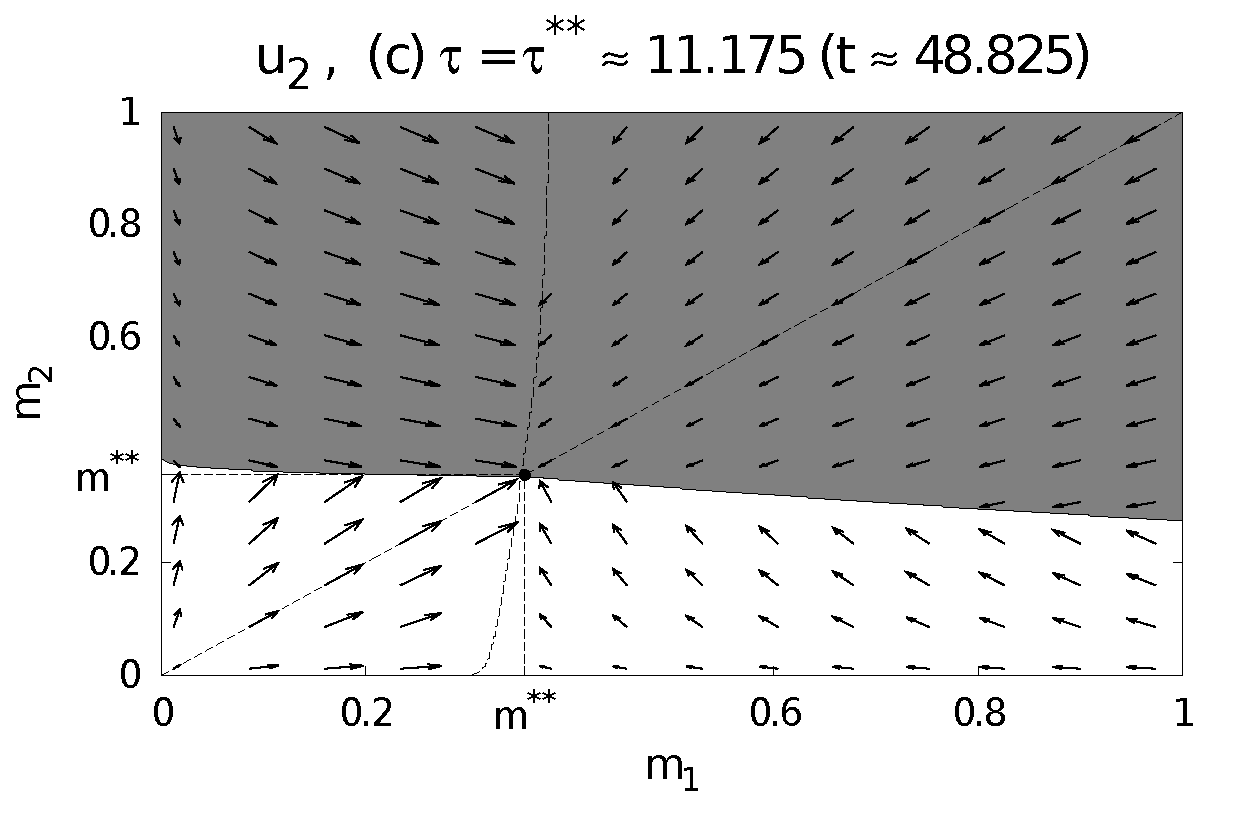
\includegraphics[width = 0.48 \textwidth]{figures/Figure_5c_2.pdf} \\
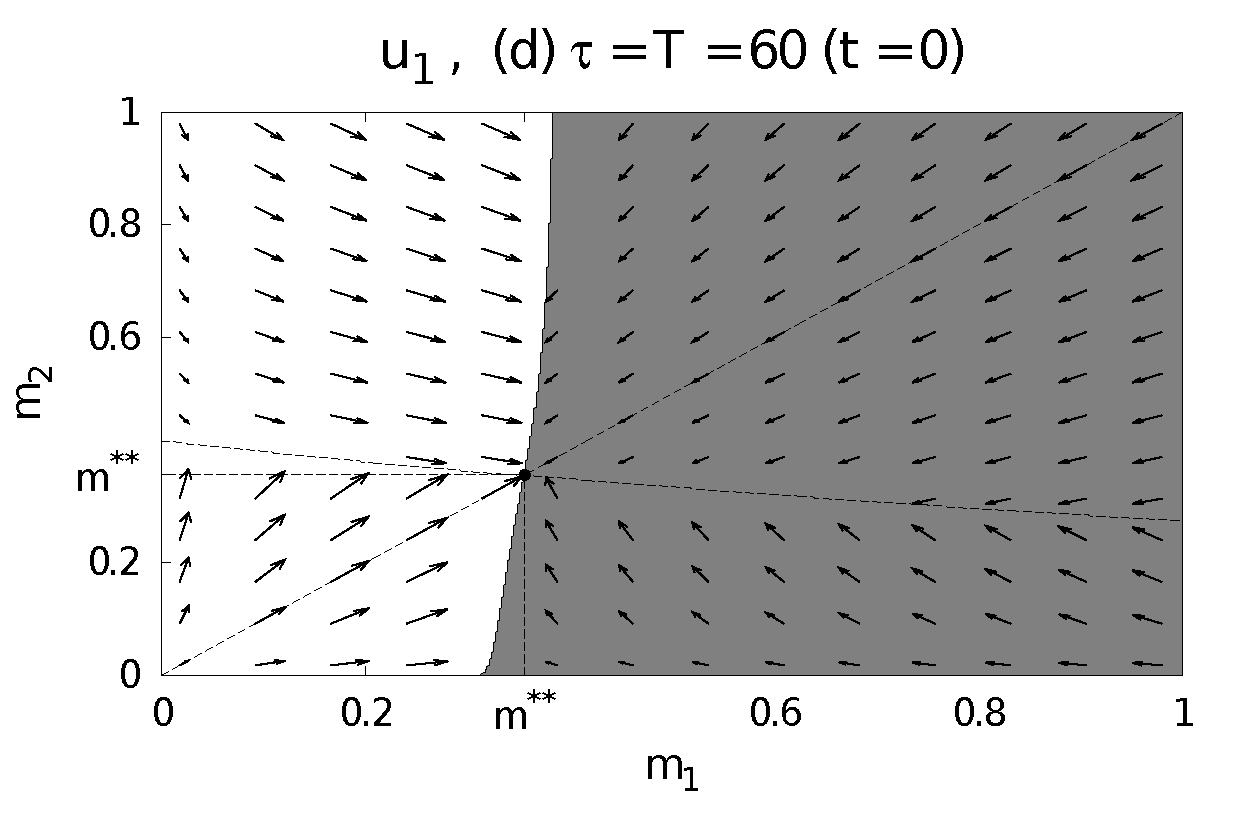
\includegraphics[width = 0.48 \textwidth]{figures/Figure_5d_1.pdf}
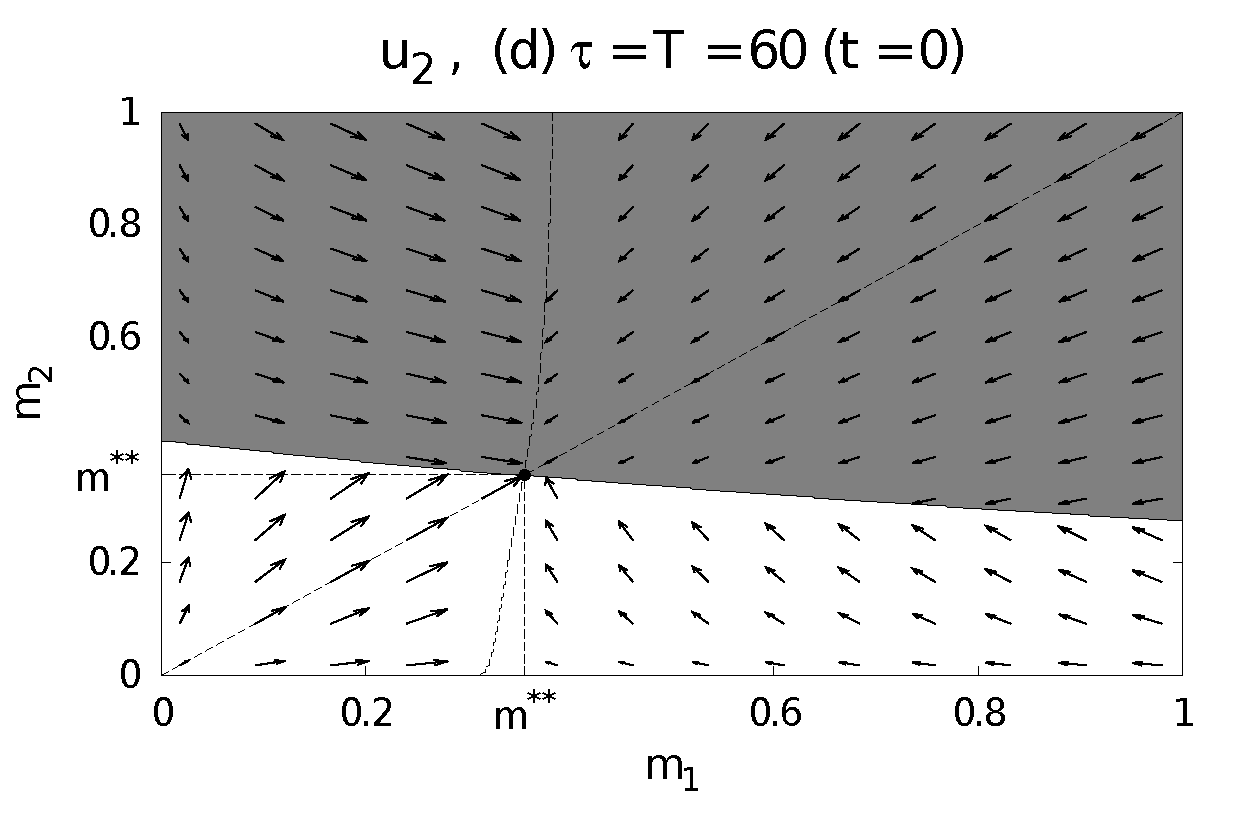
\includegraphics[width = 0.48 \textwidth]{figures/Figure_5d_2.pdf}
}
\bf \caption{\it Finite-difference approximations of the saddle feedback
control strategies at several time instants. White and gray colors show the
regions of the control values $ 0 $ and $ 1 ${\rm ,} respectively. Also
illustrated are the fields of the corresponding forward-time velocities.}
\label{Fig_5}
\end{figure}

Fig.~\ref{Fig_5} illustrates the appearance and time evolution of four
approximate switching curves. For $ \tau \geqslant \tau^{**} $, they intersect
at the point~$ \: \left( m^{**}, m^{**} \right) \, = \, 10^{-4}
\cdot \left( M^{**}, M^{**} \right) $. With the further increase of $ \tau $, the 
feedback control portrait %todo: reword and describe better
approaches a stationary form. Fig.~\ref{Fig_7}
is a three-dimensional portrait %todo: use something other than portrait
of the 
four control switching surfaces. %todo: what is a four control switching surface, define and cite
For $ \tau \geqslant \tau^{**} $, the point~$ \left( m^{**}, m^{**} \right) $
attracts forward-time trajectories and determines a steady-state equilibrium
regime for both cohorts, while one can interpret the four surfaces as turnpikes.

%todo: describe what is happening in the figures
\begin{figure}
\center{ 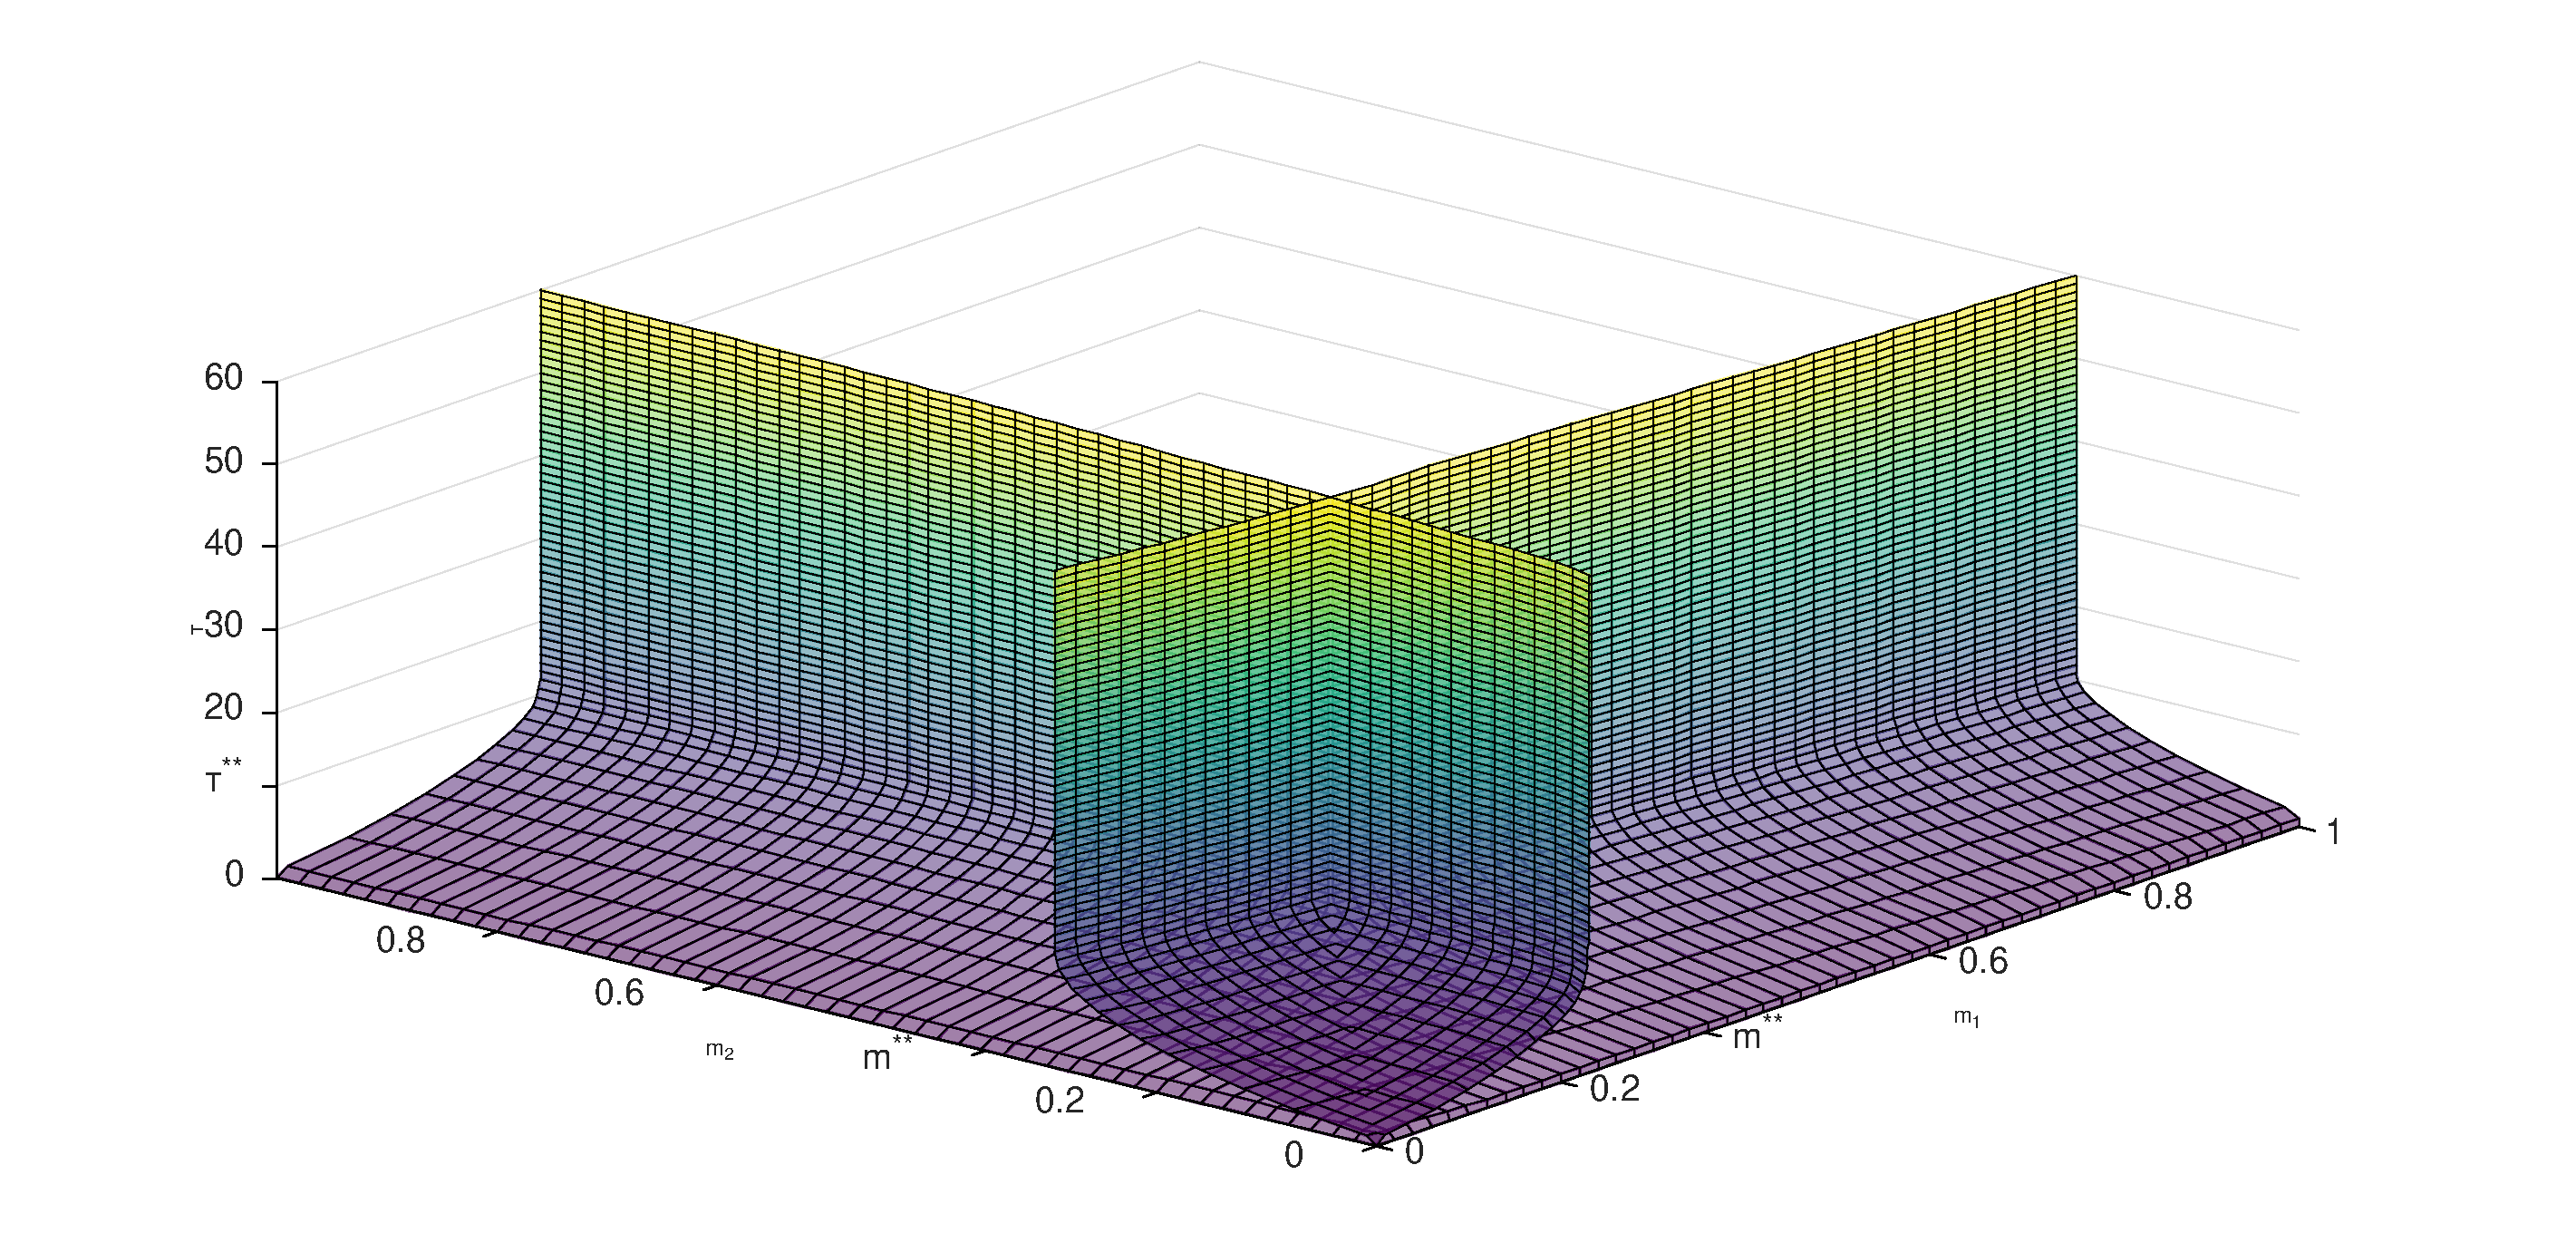
\includegraphics[width = 0.98 \textwidth]{figures/Figure_7.pdf} }
\bf \caption{\it The four control switching surfaces in the three-dimensional
space~$ (m_1, m_2, \tau) $.}
\label{Fig_7}
\end{figure}

From Fig.~{\rm \ref{Fig_4}d,} one can see that{\rm ,} in the considered domain
of initial states{\rm ,} the value $ V \left( 0, M_1^0, M_2^0 \right) $ of
the zero-sum feedback differential game is negative for $ M_1^0 > M_2^0 ${\rm ,}
zero for $ M_1^0 = M_2^0 ${\rm ,} and positive for $ M_1^0 < M_2^0 $. The
saddle feedback resource allocation strategy of cohort~{\rm 1} is uninvadable
if $ M_1^0 \geqslant M_2^0 $. Similarly{\rm ,} the saddle feedback resource
allocation strategy of cohort~{\rm 2} is uninvadable if $ M_1^0
\leqslant M_2^0 $.


\section{Conclusion}
%todo: reword the conclusion so it is not as heavily technical

The current report discusses a mathematical development that allows for constructing 
benchmark pathogenic resource allocation strategies %todo: explain more fully and provide desciption before mentioning it.
against which
we may compare actual infection mechanisms.

We have studied resource allocation equilibrium for the one-seasonal dynamics
of two biotrophic fungal cohorts within a shared host plant. It is also relevant
to investigate 
long-seasonal dynamics %todo: define or replace with something more descriptive
and 
associated evolutionary equilibria %todo: replace with something that is more understandable
of
competing pathogen cohorts. One may exploit specific discrete rules to
transition from one season to another \cite{MailleretLemesle2009,Akhmetzhanov2012}.
Another important research direction is to characterize such equilibria
themselves and whether they represent evolutionary attractors or not and how the
situation may change through evolution.

\appendix

\section{Common terms}\label{terms}
\begin{enumerate}
    \item\label{term:zerosum} \textbf{Zero-sum feedback game}: 
    \item\label{term:pathogen} \textbf{Pathogen}: this is an infectious organism, this paper mostly discusses fungal invaders.
    \item\label{term:resident} \textbf{Resident pathogen}: this is the original organism and has not been mutated.
    \item\label{term:mutant} \textbf{Mutant pathogen}: this is a strain of the same species of organism as the resident species, but has been mutated, through physical separation or natural mutation.
    \item\label{term:mycelia} \textbf{Mycelia}: the ``roots'' of a fungus, made of extremely fine branches called hyphae. 
    \item\label{term:cohort} \textbf{Cohort}: cohort typically means a person or thing that is typically on ``your side''. In this paper it typically refers to a pathogen that belongs to the same species, but differs slightly and is not of the same organism.
    \item\label{term:biotrohpic} \textbf{Biotrophic}: describes a parasite attached to plant. Describing a plant parasite.
    \item\label{term:nutrientflux} \textbf{Nutrient flux}: the amount of nutrients consumed by the pathogen.
    \item\label{term:cauchy} \textbf{The Cauchy problem}
    \item\label{term:differentialgame} \textbf{Differential game's value}:
    \item\label{term:marginal} \textbf{Two marginal fitness criteria}:
    \item\label{term:nonlinearODE} \textbf{Nonlinear ordinary differential equations}:
    \item\label{term:statevariables} \textbf{State Variables}:
    \item\label{term:saddlecontrol} \textbf{Saddle control strategies}:
    \item\label{term:carryingcapacity} \textbf{Carrying capacity}:
    
\end{enumerate}
%%%%%%%%%%%%%%%%%%%%%%%%%%%%%%%%%%%%%%%%%%%%%%1
\section{Useful Mathematical Definitions}\label{mathdefs}
\begin{enumerate}
    \item\label{math:jacobi} \textbf{Jacobi}
    \item\label{math:infimum} \textbf{Infimum}:
    \item\label{math:supremum} \textbf{Supremum}:
    \item\label{math:Argmaxmin} \textbf{Argmin/Argmax}:
    \item\label{math:saddlepoint} \textbf{Saddle point}:
    \item\label{math:maximinminimax} \textbf{Maximin / Minimax}:
    \item\label{math:valuefunction} \textbf{Value function}:
    \item\label{math:cauchyproblem} \textbf{Cauchy problem}:
    \item\label{math:nonsmooth} \textbf{Non-smooth}:
    \item\label{math:viscosity} \textbf{Viscosity}:
    \item\label{math:lipschitz} \textbf{Lipschitz continuous}:
    \item\label{math:rademacher} \textbf{Rademacher's theorem}:
    \item\label{math:lebesgue} \textbf{Lebesgue measure}:
\end{enumerate}

\section{}\label{appendix:references}Appendix
\begin{thebibliography}{}

\bibitem{YegorovGrognardMailleretHalkettBernhard2019}
I.~Yegorov, F.~Grognard, L.~Mailleret, F.~Halkett, P.~Bernhard. A dynamic game
approach to uninvadable strategies for biotrophic
pathogens. {\it Dynamic Games and Applications} 2020; {\bf 10}(1): 257--296.

\bibitem{ROCHJ2019}
Bokanowski,~O., Desilles,~A., Zidani,~H., and Zhao,~J.
User's guide for the ROC-HJ solver: Finite Differences and Semi-Lagrangian
methods. January~21,~2019. Version 2.5.4.
URL: \url{https://uma.ensta-paristech.fr/soft/ROC-HJ}

\bibitem{BernhardGrognardMailleretAkhmetzhanov2010}
Bernhard,~P., Grognard,~F., Mailleret,~L., and Akhmetzhanov,~A.
ESS for life-history traits of cooperating consumers facing cheating mutants.
[Research Report] RR--7314, INRIA, 2010.
URL: \url{https://hal.inria.fr/inria-00491489v2}

\bibitem{DercoleRinaldi2008}
Dercole,~F. and Rinaldi,~S.
{\it Analysis of Evolutionary Processes{\rm :} The Adaptive Dynamics Approach
and Its Applications}.
Princeton University Press: Princeton, 2008.

\bibitem{FlemingSoner2006}
Fleming,~W.\,H. and Soner,~H.\,M.
{\it Controlled Markov Processes and Viscosity Solutions}.
Springer-Verlag: New York, 2006.

\bibitem{Subbotin1995}
Subbotin,~A.\,I.
{\it Generalized Solutions of First-Order PDEs{\rm :} The Dynamical
Optimization Perspective}.
Birkhauser: Boston, 1995.

\bibitem{BotkinHoffmannTurova2011}
Botkin,~N.\,D., Hoffmann,~K.-H., and Turova,~V.-L.
Stable numerical schemes for solving Hamilton--Jacobi--Bellman--Isaacs
equations.
{\it SIAM Journal on Scientific Computing} 2011; {\bf 33}(2): 992--1007.

\bibitem{OsherShu1991}
Osher,~S. and Shu,~C.-W. High order essentially non-oscillatory schemes for
Hamilton--Jacobi equations.
{\it SIAM Journal on Numerical Analysis} 1991; {\bf 28}(4): 907--922.

\bibitem{BokanForcadelZidani2010}
Bokanowski,~O., Forcadel,~N., and Zidani,~H.
Reachability and minimal times for state constrained nonlinear problems without
any controllability assumption.
{\it SIAM Journal on Control and Optimization} 2010; {\bf 48}: 4292--4316.

\bibitem{PressTeukolskyVetterlingFlannery2007}
Press,~W.\,H., Teukolsky,~S.\,A., Vetterling,~W.\,T., and Flannery,~B.\,P.
{\it Numerical Recipes{\rm :} The Art of Scientific Computing}. Cambridge
University Press: New~York, 2007.

\bibitem{Yong2015}
Yong,~J.
{\it Differential Games{\rm :} A Concise Introduction}.
World Scientific Publishing: Singapore, 2015.

\bibitem{MailleretLemesle2009}
Mailleret,~L. and Lemesle,~V.
A note on semi-discrete modelling in life sciences.
{\it Philosophical Transactions of the Royal Society A} 2009; {\bf 367}:
4779--4799.

\bibitem{Akhmetzhanov2012}
Akhmetzhanov,~A.\,R., Grognard,~F., Mailleret,~L., and Bernhard,~P.
Join forces or cheat: Evolutionary analysis of a consumer-resource system.
In {\it Advances in Dynamic Games{\rm ,}
Volume {\rm 12} of the series Annals of the International Society of Dynamic
Games}, 73--95.
Springer: New York, 2012.

\bibitem{YegorovGrognardMailleretHalkett2017}
Yegorov,~I., Grognard,~F., Mailleret,~L., Halkett,~F.
Optimal resource allocation for biotrophic plant
pathogens.
IFAC-PapersOnline 50(1):3154–3159.

\bibitem{data_ivan.h}
\raggedright Glasford, S., Yegorov, I. \textit{\texttt{data\_*.h} used by
ROC-HJ to set the problem statement.}
\url{https://raw.githubusercontent.com/stevenglasford/Seminar_NDSU_2020/main/ivan_to_2.5/data/data_user_biotroph_fungi_game.h}

\end{thebibliography}

\section{Code Snippets}

\begin{figure}
    \inputminted[
        frame=lines,
        framesep=2mm,
        baselinestretch=1.2,
        fontsize=\footnotesize,
        firstline=17, 
        lastline=20]{c}{code/data.h}
\caption{A few configuration variables needed to solve the equation using
         ROC-HJ}
\label{code:defaults}
\end{figure}

\begin{figure}
    \centering
    \inputminted[frame=lines,
        framesep=2mm,
        baselinestretch=1.2,
        fontsize=\footnotesize,
        firstline=156, 
        lastline=176]{c}{code/data.h}
    \caption{Function in C++ written for ROC-HJ describing the distributed
             cost equation.}
    \label{code:cost}
\end{figure}

\begin{figure}
    \centering
    \inputminted[frame=lines,
        framesep=2mm,
        baselinestretch=1.2,
        fontsize=\footnotesize,
        firstline=133, 
        lastline=154]{c}{code/data.h}
    \caption{A C++ function for use by ROC-HJ to describe the required
             dynamic equation.}
    \label{code:dynamic}
\end{figure}

\hspace{1in}

\noindent


\end{document}
